\documentclass[11pt,compress,t,notes=noshow, xcolor=table]{beamer}
\usepackage[]{graphicx}\usepackage[]{color}
% maxwidth is the original width if it is less than linewidth
% otherwise use linewidth (to make sure the graphics do not exceed the margin)
\makeatletter
\def\maxwidth{ %
  \ifdim\Gin@nat@width>\linewidth
    \linewidth
  \else
    \Gin@nat@width
  \fi
}
\makeatother

\definecolor{fgcolor}{rgb}{0.345, 0.345, 0.345}
\newcommand{\hlnum}[1]{\textcolor[rgb]{0.686,0.059,0.569}{#1}}%
\newcommand{\hlstr}[1]{\textcolor[rgb]{0.192,0.494,0.8}{#1}}%
\newcommand{\hlcom}[1]{\textcolor[rgb]{0.678,0.584,0.686}{\textit{#1}}}%
\newcommand{\hlopt}[1]{\textcolor[rgb]{0,0,0}{#1}}%
\newcommand{\hlstd}[1]{\textcolor[rgb]{0.345,0.345,0.345}{#1}}%
\newcommand{\hlkwa}[1]{\textcolor[rgb]{0.161,0.373,0.58}{\textbf{#1}}}%
\newcommand{\hlkwb}[1]{\textcolor[rgb]{0.69,0.353,0.396}{#1}}%
\newcommand{\hlkwc}[1]{\textcolor[rgb]{0.333,0.667,0.333}{#1}}%
\newcommand{\hlkwd}[1]{\textcolor[rgb]{0.737,0.353,0.396}{\textbf{#1}}}%
\let\hlipl\hlkwb

\usepackage{framed}
\makeatletter
\newenvironment{kframe}{%
 \def\at@end@of@kframe{}%
 \ifinner\ifhmode%
  \def\at@end@of@kframe{\end{minipage}}%
  \begin{minipage}{\columnwidth}%
 \fi\fi%
 \def\FrameCommand##1{\hskip\@totalleftmargin \hskip-\fboxsep
 \colorbox{shadecolor}{##1}\hskip-\fboxsep
     % There is no \\@totalrightmargin, so:
     \hskip-\linewidth \hskip-\@totalleftmargin \hskip\columnwidth}%
 \MakeFramed {\advance\hsize-\width
   \@totalleftmargin\z@ \linewidth\hsize
   \@setminipage}}%
 {\par\unskip\endMakeFramed%
 \at@end@of@kframe}
\makeatother

\definecolor{shadecolor}{rgb}{.97, .97, .97}
\definecolor{messagecolor}{rgb}{0, 0, 0}
\definecolor{warningcolor}{rgb}{1, 0, 1}
\definecolor{errorcolor}{rgb}{1, 0, 0}
\newenvironment{knitrout}{}{} % an empty environment to be redefined in TeX

\usepackage{alltt}
\newcommand{\SweaveOpts}[1]{}  % do not interfere with LaTeX
\newcommand{\SweaveInput}[1]{} % because they are not real TeX commands
\newcommand{\Sexpr}[1]{}       % will only be parsed by R



\usepackage[english]{babel}
\usepackage[utf8]{inputenc}

\usepackage{dsfont}
\usepackage{verbatim}
\usepackage{amsmath}
\usepackage{amsfonts}
\usepackage{bm}
\usepackage{csquotes}
\usepackage{multirow}
\usepackage{longtable}
\usepackage{booktabs}
\usepackage{enumerate}
\usepackage[absolute,overlay]{textpos}
\usepackage{psfrag}
\usepackage{algorithm}
\usepackage{algpseudocode}
\usepackage{eqnarray}
\usepackage{arydshln}
\usepackage{tabularx}
\usepackage{placeins}
\usepackage{tikz}
\usepackage{setspace}
\usepackage{colortbl}
\usepackage{mathtools}
\usepackage{wrapfig}
\usepackage{bm}
\usetikzlibrary{shapes,arrows,automata,positioning,calc,chains,trees, shadows}
\tikzset{
  %Define standard arrow tip
  >=stealth',
  %Define style for boxes
  punkt/.style={
    rectangle,
    rounded corners,
    draw=black, very thick,
    text width=6.5em,
    minimum height=2em,
    text centered},
  % Define arrow style
  pil/.style={
    ->,
    thick,
    shorten <=2pt,
    shorten >=2pt,}
}
\usepackage{subfig}


% Defines macros and environments

% basic latex stuff
\newcommand{\pkg}[1]{{\fontseries{b}\selectfont #1}} %fontstyle for R packages
\newcommand{\lz}{\vspace{0.5cm}} %vertical space
\newcommand{\dlz}{\vspace{1cm}} %double vertical space
\newcommand{\mat}[1]{ %short pmatrix command
  \begin{pmatrix}
    #1
  \end{pmatrix}
}
\newcommand{\oneliner}[1] % Oneliner for important statements
{\begin{block}{}\begin{center}\begin{Large}#1\end{Large}\end{center}\end{block}}


% 
% basic latex stuff
\newcommand{\pkg}[1]{{\fontseries{b}\selectfont #1}} %fontstyle for R packages
\newcommand{\lz}{\vspace{0.5cm}} %vertical space
\newcommand{\dlz}{\vspace{1cm}} %double vertical space
\newcommand{\mat}[1]{ %short pmatrix command
  \begin{pmatrix}
    #1
  \end{pmatrix}
}
\newcommand{\oneliner}[1] % Oneliner for important statements
{\begin{block}{}\begin{center}\begin{Large}#1\end{Large}\end{center}\end{block}}



%\usetheme{lmu-lecture}
\usepackage{../../style/lmu-lecture}

\let\code=\texttt
\let\proglang=\textsf

\setkeys{Gin}{width=0.9\textwidth}

\title{Introduction to Machine Learning}
% \author{Bernd Bischl, Christoph Molnar, Daniel Schalk, Fabian Scheipl}
\institute{\href{https://compstat-lmu.github.io/lecture_i2ml/}{compstat-lmu.github.io/lecture\_i2ml}}
\date{}

\setbeamertemplate{frametitle}{\expandafter\uppercase\expandafter\insertframetitle}



\begin{document}
% Introduction to Machine Learning
% Day 4

% Set style/preamble.Rnw as parent.


% Load all R packages and set up knitr

% This file loads R packages, configures knitr options and sets preamble.Rnw as parent file
% IF YOU MODIFY THIS, PLZ ALSO MODIFY setup.Rmd ACCORDINGLY...








% Defines macros and environments
% ml - trees, extra trees

\newcommand{\Np}{\mathcal{N}}												% Parent node N
\newcommand{\Nl}{\Np_1}														% Left node N_1
\newcommand{\Nr}{\Np_2}														% Right node N_2

% ml - bagging, random forest

\newcommand{\bl}[1]{b^{[#1]}(x)}											% baselearner with argument for m
\newcommand{\blm}{\bl{m}}												    % baselearner without argument for m
\newcommand{\blmh}{\hat{b}^{[m]}(x)}										% estimated base learner 


%! includes: forests-intro


\lecturechapter{Random Forests: Feature Importance}
\lecture{Introduction to Machine Learning}

\sloppy


\begin{vbframe}{Variable Importance}

\begin{itemize}
  \item Single trees are highly interpretable
  \item Random Forests as ensembles of trees lose this feature
  \item Contributions of the different features to the model are difficult to evaluate
  \item Way out: variable importance measures
  \item Basic idea: by how much would performance of the random forest decrease if a specific feature were removed or rendered useless?
\end{itemize}


\framebreak

\begin{algorithm}[H]
  \small
  \caption*{Measure based on improvement in split criterion}
  \begin{algorithmic}[0]
    \For{features $x_j$, $j = 1$ to $p$}
    \For{tree base learners $\blmh$, $m = 1$ to $M$}
    \State {Find all nodes $\Np$ in $\blmh$ that use $x_j$.} 
    \State {Compute improvement in splitting criterion achieved by them.}
    \State {Add up these improvements.}
    \EndFor
    \State {Add up improvements over all trees to get feature importance of $x_j$.}
    %\State {This is the feature importance for $x_j$.}
    \EndFor
  \end{algorithmic}
\end{algorithm}
\vskip -2em
\begin{figure}
\begin{knitrout}\footnotesize
\definecolor{shadecolor}{rgb}{0.969, 0.969, 0.969}\color{fgcolor}

{\centering 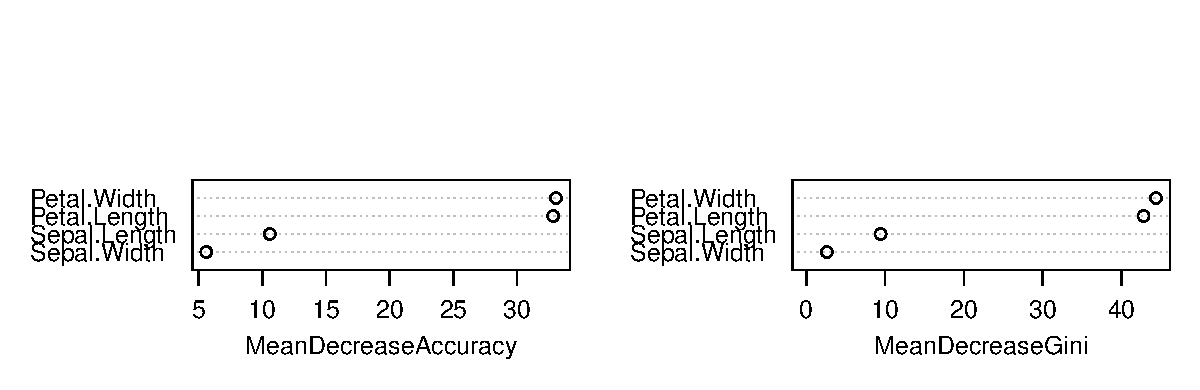
\includegraphics[width=0.95\textwidth]{figure/cart_forest_fimp_1} 

}



\end{knitrout}
% \caption{Two importance measures on the iris dataset.}
\end{figure}

\framebreak

\begin{algorithm}[H]
  \small
  \caption*{Measure based on permutations of OOB observations}
  \begin{algorithmic}[0]
    \State While growing tree, pass down OOB observations and record predictive accuracy.
    \State Permute OOB observations of $j$-th feature. This destroys the association between the target and the permuted $j$-th feature.
    \State Pass down the permuted OOB observations and evaluate predictive accuracy again.
    \State The decrease of performance induced by permutation is averaged over all trees and
  is used as a measure for the importance of the $j$-th variable.
  \end{algorithmic}
\end{algorithm}

% \framebreak

% <<>>=
% lrn = makeLearner("classif.randomForest", importance = TRUE)
% mod = train(lrn, iris.task)
% mlr::getFeatureImportance(mod)
% @

% \framebreak

% <<echo=TRUE, size="footnotesize", fig.height=4>>=
% rf = getLearnerModel(mod)
% randomForest::varImpPlot(rf,
%   main = "Variable Importance")
% @

% \framebreak

% <<echo=TRUE, size="footnotesize", fig.height=4>>=
% v = generateFilterValuesData(iris.task,
%   method = c("rf.importance", "cforest.importance"))
% plotFilterValues(v)
% @


\end{vbframe}

\begin{vbframe}{Variable Importance based on permutations of OOB observations}
\begin{center}
% FIGURE SOURCE: https://docs.google.com/presentation/d/16gg9PqtEV_Ii_ZBw0zA9GdUIled-6OVkoqArX1ouTmo/edit#slide=id.p
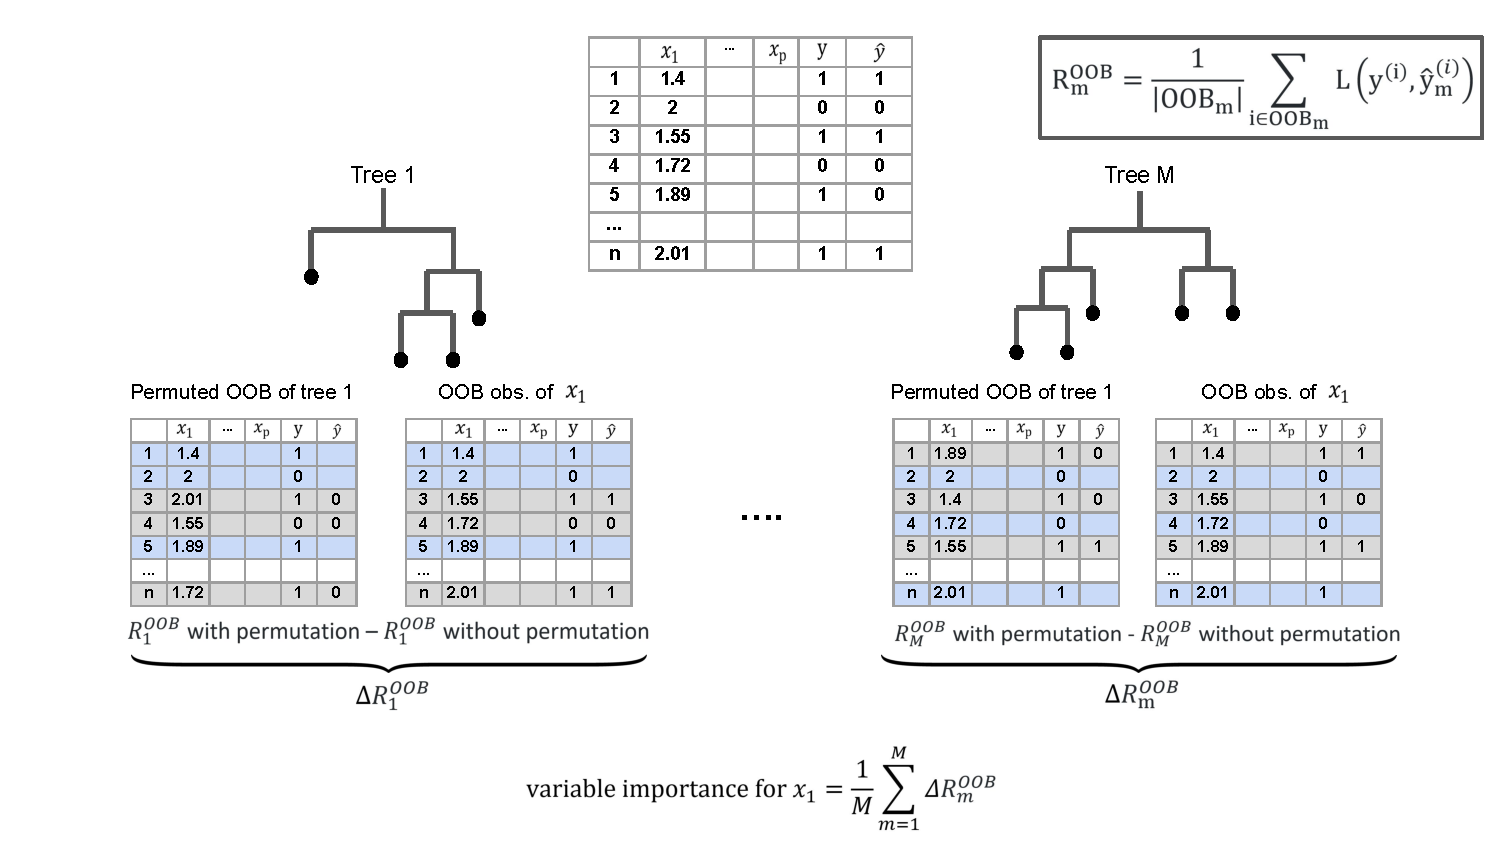
\includegraphics[width = 10.3cm]{figure_man/rF_varImp_permutation_new.pdf}
\end{center}
\end{vbframe}

\endlecture
\end{document}
